\documentclass[a4paper]{book}
\usepackage{a4wide}
\usepackage{makeidx}
\usepackage{fancyhdr}
\usepackage{graphicx}
\usepackage{multicol}
\usepackage{float}
\usepackage{textcomp}
\usepackage{alltt}
\usepackage{times}
\usepackage{ifpdf}
\ifpdf
\usepackage[pdftex,
            pagebackref=true,
            colorlinks=true,
            linkcolor=blue
           ]{hyperref}
\else
\usepackage[ps2pdf,
            pagebackref=true,
            colorlinks=true,
            linkcolor=blue
           ]{hyperref}
\usepackage{pspicture}
\fi
\usepackage{doxygen}
\makeindex
\setcounter{tocdepth}{1}
\renewcommand{\footrulewidth}{0.4pt}
\begin{document}
\begin{titlepage}
\vspace*{7cm}
\begin{center}
{\Large Paradis\-EO-PEO: Parallel and Distributed Evolving Objects - Lessons Reference Manual\\[1ex]\large 1.0 }\\
\vspace*{1cm}
{\large Generated by Doxygen 1.4.7}\\
\vspace*{0.5cm}
{\small Fri Oct 12 15:06:31 2007}\\
\end{center}
\end{titlepage}
\clearemptydoublepage
\pagenumbering{roman}
\tableofcontents
\clearemptydoublepage
\pagenumbering{arabic}
\chapter{Paradis\-EO-PEO: Parallel and Distributed Evolving Objects - Lessons Hierarchical Index}
\section{Paradis\-EO-MO-Moving\-Objects Class Hierarchy}
This inheritance list is sorted roughly, but not completely, alphabetically:\begin{CompactList}
\item eo\-Functor\-Base{\tt  [external]}\begin{CompactList}
\item eo\-BF$<$ const EOT \&, const EOT \&, bool $>${\tt  [external]}\begin{CompactList}
\item \contentsline{section}{mo\-Comparator$<$ EOT $>$}{\pageref{classmo_comparator}}{}
\begin{CompactList}
\item \contentsline{section}{mo\-Fit\-Comparator$<$ EOT $>$}{\pageref{classmo_fit_comparator}}{}
\end{CompactList}
\end{CompactList}
\item eo\-BF$<$ const M \&, const M::EOType \&, bool $>${\tt  [external]}\begin{CompactList}
\item \contentsline{section}{mo\-Tabu\-List$<$ M $>$}{\pageref{classmo_tabu_list}}{}
\begin{CompactList}
\item \contentsline{section}{mo\-Simple\-Move\-Tabu\-List$<$ M $>$}{\pageref{classmo_simple_move_tabu_list}}{}
\item \contentsline{section}{mo\-Simple\-Solution\-Tabu\-List$<$ M $>$}{\pageref{classmo_simple_solution_tabu_list}}{}
\end{CompactList}
\end{CompactList}
\item eo\-BF$<$ const M \&, const M::EOType \&, M::EOType::Fitness $>${\tt  [external]}\begin{CompactList}
\item \contentsline{section}{mo\-Move\-Incr\-Eval$<$ M $>$}{\pageref{classmo_move_incr_eval}}{}
\end{CompactList}
\item eo\-BF$<$ const M \&, const M::EOType \&, void $>${\tt  [external]}\begin{CompactList}
\item \contentsline{section}{mo\-LSCheck\-Point$<$ M $>$}{\pageref{classmo_l_s_check_point}}{}
\end{CompactList}
\item eo\-BF$<$ const M \&, const M::EOType::Fitness \&, bool $>${\tt  [external]}\begin{CompactList}
\item \contentsline{section}{mo\-Aspir\-Crit$<$ M $>$}{\pageref{classmo_aspir_crit}}{}
\begin{CompactList}
\item \contentsline{section}{mo\-Impr\-Best\-Fit\-Aspir\-Crit$<$ M $>$}{\pageref{classmo_impr_best_fit_aspir_crit}}{}
\item \contentsline{section}{mo\-No\-Aspir\-Crit$<$ M $>$}{\pageref{classmo_no_aspir_crit}}{}
\end{CompactList}
\end{CompactList}
\item eo\-BF$<$ const M::EOType \&, M::EOType \&, void $>${\tt  [external]}\begin{CompactList}
\item \contentsline{section}{mo\-Move\-Expl$<$ M $>$}{\pageref{classmo_move_expl}}{}
\begin{CompactList}
\item \contentsline{section}{mo\-Move\-Loop\-Expl$<$ M $>$}{\pageref{classmo_move_loop_expl}}{}
\begin{CompactList}
\item \contentsline{section}{mo\-HCMove\-Loop\-Expl$<$ M $>$}{\pageref{classmo_h_c_move_loop_expl}}{}
\item \contentsline{section}{mo\-TSMove\-Loop\-Expl$<$ M $>$}{\pageref{classmo_t_s_move_loop_expl}}{}
\end{CompactList}
\end{CompactList}
\end{CompactList}
\item eo\-BF$<$ M \&, const M::EOType \&, bool $>${\tt  [external]}\begin{CompactList}
\item \contentsline{section}{mo\-Next\-Move$<$ M $>$}{\pageref{classmo_next_move}}{}
\begin{CompactList}
\item \contentsline{section}{mo\-It\-Rand\-Next\-Move$<$ M $>$}{\pageref{classmo_it_rand_next_move}}{}
\end{CompactList}
\end{CompactList}
\item eo\-BF$<$ M \&, const M::EOType \&, void $>${\tt  [external]}\begin{CompactList}
\item \contentsline{section}{mo\-Move\-Init$<$ M $>$}{\pageref{classmo_move_init}}{}
\end{CompactList}
\item eo\-BF$<$ M \&, M::EOType::Fitness \&, void $>${\tt  [external]}\begin{CompactList}
\item \contentsline{section}{mo\-Move\-Select$<$ M $>$}{\pageref{classmo_move_select}}{}
\begin{CompactList}
\item \contentsline{section}{mo\-Best\-Impr\-Select$<$ M $>$}{\pageref{classmo_best_impr_select}}{}
\item \contentsline{section}{mo\-First\-Impr\-Select$<$ M $>$}{\pageref{classmo_first_impr_select}}{}
\item \contentsline{section}{mo\-Rand\-Impr\-Select$<$ M $>$}{\pageref{classmo_rand_impr_select}}{}
\end{CompactList}
\end{CompactList}
\item eo\-UF$<$ const EOT \&, bool $>${\tt  [external]}\begin{CompactList}
\item \contentsline{section}{mo\-Sol\-Continue$<$ EOT $>$}{\pageref{classmo_sol_continue}}{}
\begin{CompactList}
\item \contentsline{section}{mo\-Fit\-Sol\-Continue$<$ EOT $>$}{\pageref{classmo_fit_sol_continue}}{}
\item \contentsline{section}{mo\-Gen\-Sol\-Continue$<$ EOT $>$}{\pageref{classmo_gen_sol_continue}}{}
\item \contentsline{section}{mo\-No\-Fit\-Impr\-Sol\-Continue$<$ EOT $>$}{\pageref{classmo_no_fit_impr_sol_continue}}{}
\item \contentsline{section}{mo\-Steady\-Fit\-Sol\-Continue$<$ EOT $>$}{\pageref{classmo_steady_fit_sol_continue}}{}
\end{CompactList}
\end{CompactList}
\item eo\-UF$<$ double \&, bool $>${\tt  [external]}\begin{CompactList}
\item \contentsline{section}{mo\-Cooling\-Schedule}{\pageref{classmo_cooling_schedule}}{}
\begin{CompactList}
\item \contentsline{section}{mo\-Exponential\-Cooling\-Schedule}{\pageref{classmo_exponential_cooling_schedule}}{}
\item \contentsline{section}{mo\-Linear\-Cooling\-Schedule}{\pageref{classmo_linear_cooling_schedule}}{}
\end{CompactList}
\end{CompactList}
\item eo\-UF$<$ EOT \&, bool $>${\tt  [external]}\begin{CompactList}
\item eo\-Mon\-Op$<$ EOT $>${\tt  [external]}\begin{CompactList}
\item \contentsline{section}{mo\-Algo$<$ EOT $>$}{\pageref{classmo_algo}}{}
\end{CompactList}
\end{CompactList}
\item eo\-UF$<$ EOT \&, void $>${\tt  [external]}\begin{CompactList}
\item \contentsline{section}{mo\-Move$<$ EOT $>$}{\pageref{classmo_move}}{}
\end{CompactList}
\item eo\-UF$<$ EOType \&, bool $>${\tt  [external]}\item eo\-UF$<$ M \&, void $>${\tt  [external]}\begin{CompactList}
\item \contentsline{section}{mo\-Rand\-Move$<$ M $>$}{\pageref{classmo_rand_move}}{}
\end{CompactList}
\item eo\-UF$<$ M::EOType \&, bool $>${\tt  [external]}\begin{CompactList}
\item eo\-Mon\-Op$<$ M::EOType $>${\tt  [external]}\begin{CompactList}
\item \contentsline{section}{mo\-Algo$<$ M::EOType $>$}{\pageref{classmo_algo}}{}
\begin{CompactList}
\item \contentsline{section}{mo\-HC$<$ M $>$}{\pageref{classmo_h_c}}{}
\item \contentsline{section}{mo\-ILS$<$ M $>$}{\pageref{classmo_i_l_s}}{}
\item \contentsline{section}{mo\-SA$<$ M $>$}{\pageref{classmo_s_a}}{}
\item \contentsline{section}{mo\-TS$<$ M $>$}{\pageref{classmo_t_s}}{}
\end{CompactList}
\end{CompactList}
\end{CompactList}
\end{CompactList}
\item eo\-Op$<$ EOType $>${\tt  [external]}\begin{CompactList}
\item eo\-Mon\-Op$<$ EOT $>${\tt  [external]}\item eo\-Mon\-Op$<$ M::EOType $>${\tt  [external]}\end{CompactList}
\end{CompactList}

\chapter{Paradis\-EO-PEO: Parallel and Distributed Evolving Objects - Lessons Class Index}
\section{ParadisEO-MOMovingObjects Class List}
Here are the classes, structs, unions and interfaces with brief descriptions:\begin{CompactList}
\item\contentsline{section}{{\bf EmptySelection} (Special class that describes the case of no selection )}{\pageref{class_empty_selection}}{}
\item\contentsline{section}{{\bf moAlgo$<$ EOT $>$} (Description of an algorithm of the paradiseo-mo library )}{\pageref{classmo_algo}}{}
\item\contentsline{section}{{\bf moAspirCrit$<$ M $>$} (Description of the conditions in which a tabu move could be accepted )}{\pageref{classmo_aspir_crit}}{}
\item\contentsline{section}{{\bf moBestImprSelect$<$ M $>$} (One of the possible \doxyref{moMoveSelect}{p.}{classmo_move_select} )}{\pageref{classmo_best_impr_select}}{}
\item\contentsline{section}{{\bf moComparator$<$ EOT $>$} (Template for classes which need to compare two EOT and indicate if the first is \char`\"{}better\char`\"{} than the second )}{\pageref{classmo_comparator}}{}
\item\contentsline{section}{{\bf moCoolingSchedule} (This class gives the description of a cooling schedule )}{\pageref{classmo_cooling_schedule}}{}
\item\contentsline{section}{{\bf moExponentialCoolingSchedule} (One of the possible \doxyref{moCoolingSchedule}{p.}{classmo_cooling_schedule} )}{\pageref{classmo_exponential_cooling_schedule}}{}
\item\contentsline{section}{{\bf moFirstImprSelect$<$ M $>$} (One possible \doxyref{moMoveSelect}{p.}{classmo_move_select} )}{\pageref{classmo_first_impr_select}}{}
\item\contentsline{section}{{\bf moFitComparator$<$ EOT $>$} (Comparison according to the fitness )}{\pageref{classmo_fit_comparator}}{}
\item\contentsline{section}{{\bf moFitSolContinue$<$ EOT $>$} (One possible stop criterion for a solution-based heuristic )}{\pageref{classmo_fit_sol_continue}}{}
\item\contentsline{section}{{\bf moGenSolContinue$<$ EOT $>$} (One possible stop criterion for a solution-based heuristic )}{\pageref{classmo_gen_sol_continue}}{}
\item\contentsline{section}{{\bf moHC$<$ M $>$} (Hill Climbing (HC) )}{\pageref{classmo_h_c}}{}
\item\contentsline{section}{{\bf moHCMoveLoopExpl$<$ M $>$} (Iterative explorer used by a \doxyref{moHC}{p.}{classmo_h_c} )}{\pageref{classmo_h_c_move_loop_expl}}{}
\item\contentsline{section}{{\bf moILS$<$ M $>$} (Iterated Local Search (ILS) )}{\pageref{classmo_i_l_s}}{}
\item\contentsline{section}{{\bf moImprBestFitAspirCrit$<$ M $>$} (One of the possible \doxyref{moAspirCrit}{p.}{classmo_aspir_crit} )}{\pageref{classmo_impr_best_fit_aspir_crit}}{}
\item\contentsline{section}{{\bf moItRandNextMove$<$ M $>$} (One of the possible \doxyref{moNextMove}{p.}{classmo_next_move} )}{\pageref{classmo_it_rand_next_move}}{}
\item\contentsline{section}{{\bf moLinearCoolingSchedule} (One of the possible \doxyref{moCoolingSchedule}{p.}{classmo_cooling_schedule} )}{\pageref{classmo_linear_cooling_schedule}}{}
\item\contentsline{section}{{\bf moLSCheckPoint$<$ M $>$} (Class which allows a checkpointing system )}{\pageref{classmo_l_s_check_point}}{}
\item\contentsline{section}{{\bf moMove$<$ EOT $>$} (Definition of a move )}{\pageref{classmo_move}}{}
\item\contentsline{section}{{\bf moMoveExpl$<$ M $>$} (Description of a move (\doxyref{moMove}{p.}{classmo_move}) explorer )}{\pageref{classmo_move_expl}}{}
\item\contentsline{section}{{\bf moMoveIncrEval$<$ M $>$} ((generally) Efficient evaluation function based a move and a solution )}{\pageref{classmo_move_incr_eval}}{}
\item\contentsline{section}{{\bf moMoveInit$<$ M $>$} (Move (\doxyref{moMove}{p.}{classmo_move}) initializer )}{\pageref{classmo_move_init}}{}
\item\contentsline{section}{{\bf moMoveLoopExpl$<$ M $>$} (Class which describes an iterative explorer )}{\pageref{classmo_move_loop_expl}}{}
\item\contentsline{section}{{\bf moMoveSelect$<$ M $>$} (Class that describes a move selector (\doxyref{moMove}{p.}{classmo_move}) )}{\pageref{classmo_move_select}}{}
\item\contentsline{section}{{\bf moNextMove$<$ M $>$} (Class which allows to generate a new move (\doxyref{moMove}{p.}{classmo_move}) )}{\pageref{classmo_next_move}}{}
\item\contentsline{section}{{\bf moNoAspirCrit$<$ M $>$} (One of the possible aspiration criterion (\doxyref{moAspirCrit}{p.}{classmo_aspir_crit}) )}{\pageref{classmo_no_aspir_crit}}{}
\item\contentsline{section}{{\bf moNoFitImprSolContinue$<$ EOT $>$} (One possible stop criterion for a solution-based heuristic )}{\pageref{classmo_no_fit_impr_sol_continue}}{}
\item\contentsline{section}{{\bf moRandImprSelect$<$ M $>$} (One of the possible \doxyref{moMove}{p.}{classmo_move} selector (\doxyref{moMoveSelect}{p.}{classmo_move_select}) )}{\pageref{classmo_rand_impr_select}}{}
\item\contentsline{section}{{\bf moRandMove$<$ M $>$} (Random move generator )}{\pageref{classmo_rand_move}}{}
\item\contentsline{section}{{\bf moSA$<$ M $>$} (Simulated Annealing (SA) )}{\pageref{classmo_s_a}}{}
\item\contentsline{section}{{\bf moSimpleMoveTabuList$<$ M $>$} (Class describing a move tabu list with a limited memory )}{\pageref{classmo_simple_move_tabu_list}}{}
\item\contentsline{section}{{\bf moSimpleSolutionTabuList$<$ M $>$} (Class describing a solution tabu list with limited length )}{\pageref{classmo_simple_solution_tabu_list}}{}
\item\contentsline{section}{{\bf moSolContinue$<$ EOT $>$} (Class that describes a stop criterion for a solution-based heuristic )}{\pageref{classmo_sol_continue}}{}
\item\contentsline{section}{{\bf moSteadyFitSolContinue$<$ EOT $>$} (One possible stopping criterion for a solution-based heuristic )}{\pageref{classmo_steady_fit_sol_continue}}{}
\item\contentsline{section}{{\bf moTabuList$<$ M $>$} (Class describing a tabu list that a \doxyref{moTS}{p.}{classmo_t_s} uses )}{\pageref{classmo_tabu_list}}{}
\item\contentsline{section}{{\bf moTS$<$ M $>$} (Tabu Search (TS) )}{\pageref{classmo_t_s}}{}
\item\contentsline{section}{{\bf moTSMoveLoopExpl$<$ M $>$} (Explorer for a Tabu Search algorithm )}{\pageref{classmo_t_s_move_loop_expl}}{}
\end{CompactList}

\chapter{Paradis\-EO-PEO: Parallel and Distributed Evolving Objects - Lessons Class Documentation}
\hypertarget{classCitySwap}{
\section{City\-Swap Class Reference}
\label{classCitySwap}\index{CitySwap@{CitySwap}}
}
Its swaps two vertices randomly choosen.  


{\tt \#include $<$city\_\-swap.h$>$}

Inheritance diagram for City\-Swap::\begin{figure}[H]
\begin{center}
\leavevmode
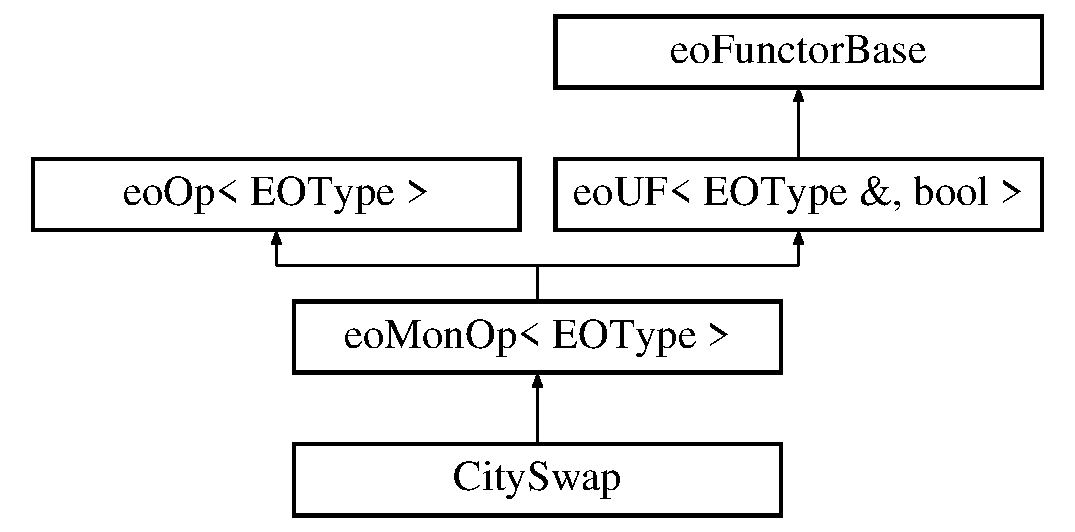
\includegraphics[height=4cm]{classCitySwap}
\end{center}
\end{figure}
\subsection*{Public Member Functions}
\begin{CompactItemize}
\item 
\hypertarget{classCitySwap_7e6958b62048c89604cbf046b86bdf2d}{
bool \hyperlink{classCitySwap_7e6958b62048c89604cbf046b86bdf2d}{operator()} (\bf{Route} \&\_\-\_\-route)}
\label{classCitySwap_7e6958b62048c89604cbf046b86bdf2d}

\end{CompactItemize}


\subsection{Detailed Description}
Its swaps two vertices randomly choosen. 



Definition at line 46 of file city\_\-swap.h.

The documentation for this class was generated from the following files:\begin{CompactItemize}
\item 
city\_\-swap.h\item 
city\_\-swap.cpp\end{CompactItemize}

\hypertarget{classDisplayBestRoute}{
\section{Display\-Best\-Route Class Reference}
\label{classDisplayBestRoute}\index{DisplayBestRoute@{DisplayBestRoute}}
}
\subsection*{Public Member Functions}
\begin{CompactItemize}
\item 
\hypertarget{classDisplayBestRoute_db263e38f1e82174f811bf62f323f87f}{
\hyperlink{classDisplayBestRoute_db263e38f1e82174f811bf62f323f87f}{Display\-Best\-Route} (eo\-Pop$<$ Route $>$ \&\_\-\_\-pop)}
\label{classDisplayBestRoute_db263e38f1e82174f811bf62f323f87f}

\item 
\hypertarget{classDisplayBestRoute_ee879344a6d8b81a04d4eabbed2c7a04}{
void \hyperlink{classDisplayBestRoute_ee879344a6d8b81a04d4eabbed2c7a04}{operator()} ()}
\label{classDisplayBestRoute_ee879344a6d8b81a04d4eabbed2c7a04}

\end{CompactItemize}
\subsection*{Private Attributes}
\begin{CompactItemize}
\item 
\hypertarget{classDisplayBestRoute_5270aabbf294d2deca9878934216eb89}{
eo\-Pop$<$ Route $>$ \& \hyperlink{classDisplayBestRoute_5270aabbf294d2deca9878934216eb89}{pop}}
\label{classDisplayBestRoute_5270aabbf294d2deca9878934216eb89}

\end{CompactItemize}


\subsection{Detailed Description}




Definition at line 18 of file display\_\-best\_\-route.h.

The documentation for this class was generated from the following files:\begin{CompactItemize}
\item 
display\_\-best\_\-route.h\item 
display\_\-best\_\-route.cpp\end{CompactItemize}

\hypertarget{classEdgeXover}{
\section{Edge\-Xover Class Reference}
\label{classEdgeXover}\index{EdgeXover@{EdgeXover}}
}
Edge Crossover.  


{\tt \#include $<$edge\_\-xover.h$>$}

Inheritance diagram for Edge\-Xover::\begin{figure}[H]
\begin{center}
\leavevmode
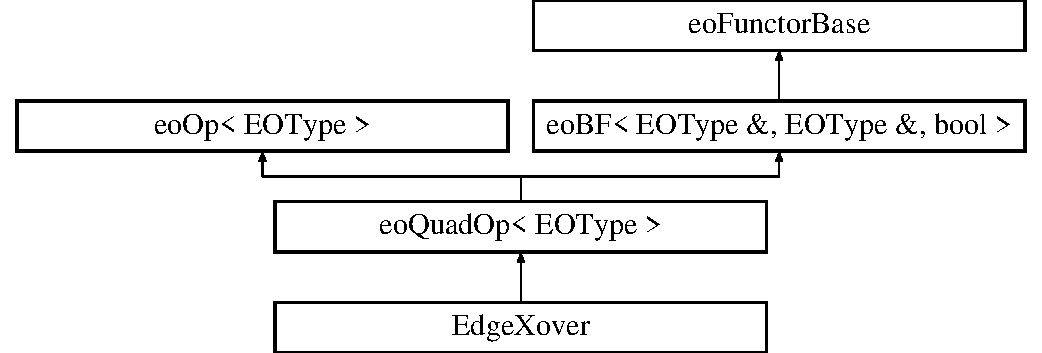
\includegraphics[height=4cm]{classEdgeXover}
\end{center}
\end{figure}
\subsection*{Public Member Functions}
\begin{CompactItemize}
\item 
\hypertarget{classEdgeXover_cb1c0a103106a4d3319540cb23163a79}{
bool \hyperlink{classEdgeXover_cb1c0a103106a4d3319540cb23163a79}{operator()} (\bf{Route} \&\_\-\_\-route1, \bf{Route} \&\_\-\_\-route2)}
\label{classEdgeXover_cb1c0a103106a4d3319540cb23163a79}

\end{CompactItemize}
\subsection*{Private Member Functions}
\begin{CompactItemize}
\item 
\hypertarget{classEdgeXover_88c2d4c9a878454a32d56010f3dddc27}{
void \hyperlink{classEdgeXover_88c2d4c9a878454a32d56010f3dddc27}{cross} (const \bf{Route} \&\_\-\_\-par1, const \bf{Route} \&\_\-\_\-par2, \bf{Route} \&\_\-\_\-child)}
\label{classEdgeXover_88c2d4c9a878454a32d56010f3dddc27}

\item 
\hypertarget{classEdgeXover_1b3a4c75dd9a034c81af6d89d85d30f5}{
void \hyperlink{classEdgeXover_1b3a4c75dd9a034c81af6d89d85d30f5}{remove\_\-entry} (unsigned \_\-\_\-vertex, std::vector$<$ std::set$<$ unsigned $>$ $>$ \&\_\-\_\-map)}
\label{classEdgeXover_1b3a4c75dd9a034c81af6d89d85d30f5}

\item 
\hypertarget{classEdgeXover_04de96aa1016836e0ba5f4b952a5fa16}{
void \hyperlink{classEdgeXover_04de96aa1016836e0ba5f4b952a5fa16}{build\_\-map} (const \bf{Route} \&\_\-\_\-par1, const \bf{Route} \&\_\-\_\-par2)}
\label{classEdgeXover_04de96aa1016836e0ba5f4b952a5fa16}

\item 
\hypertarget{classEdgeXover_2d3045ef503d8b16a27e11fdc23ca11c}{
void \hyperlink{classEdgeXover_2d3045ef503d8b16a27e11fdc23ca11c}{add\_\-vertex} (unsigned \_\-\_\-vertex, \bf{Route} \&\_\-\_\-child)}
\label{classEdgeXover_2d3045ef503d8b16a27e11fdc23ca11c}

\end{CompactItemize}
\subsection*{Private Attributes}
\begin{CompactItemize}
\item 
\hypertarget{classEdgeXover_d41399c6effb54ee48c722f1e19cb3c3}{
std::vector$<$ std::set$<$ unsigned $>$ $>$ \hyperlink{classEdgeXover_d41399c6effb54ee48c722f1e19cb3c3}{\_\-map}}
\label{classEdgeXover_d41399c6effb54ee48c722f1e19cb3c3}

\item 
\hypertarget{classEdgeXover_46d4d4724cf6d660b1a7ab4a346573d4}{
std::vector$<$ bool $>$ \hyperlink{classEdgeXover_46d4d4724cf6d660b1a7ab4a346573d4}{visited}}
\label{classEdgeXover_46d4d4724cf6d660b1a7ab4a346573d4}

\end{CompactItemize}


\subsection{Detailed Description}
Edge Crossover. 



Definition at line 48 of file edge\_\-xover.h.

The documentation for this class was generated from the following files:\begin{CompactItemize}
\item 
edge\_\-xover.h\item 
edge\_\-xover.cpp\end{CompactItemize}

\hypertarget{classMergeRouteEval}{
\section{Merge\-Route\-Eval Class Reference}
\label{classMergeRouteEval}\index{MergeRouteEval@{MergeRouteEval}}
}
Inheritance diagram for Merge\-Route\-Eval::\begin{figure}[H]
\begin{center}
\leavevmode
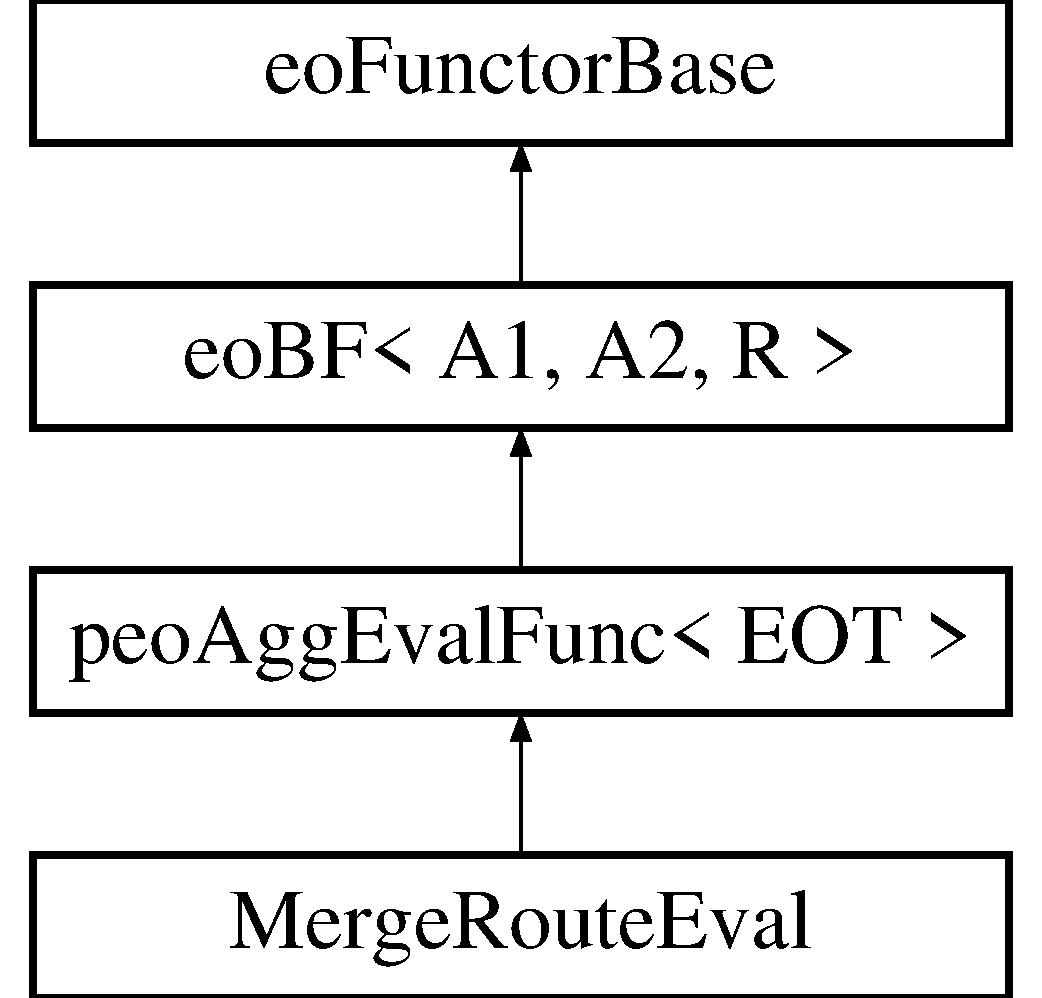
\includegraphics[height=2cm]{classMergeRouteEval}
\end{center}
\end{figure}
\subsection*{Public Member Functions}
\begin{CompactItemize}
\item 
\hypertarget{classMergeRouteEval_29cb0028ac0df4b2cee3a809c8f35dea}{
void \hyperlink{classMergeRouteEval_29cb0028ac0df4b2cee3a809c8f35dea}{operator()} (Route \&\_\-\_\-route, const int \&\_\-\_\-part\_\-fit)}
\label{classMergeRouteEval_29cb0028ac0df4b2cee3a809c8f35dea}

\end{CompactItemize}


\subsection{Detailed Description}




Definition at line 31 of file merge\_\-route\_\-eval.h.

The documentation for this class was generated from the following files:\begin{CompactItemize}
\item 
merge\_\-route\_\-eval.h\item 
merge\_\-route\_\-eval.cpp\end{CompactItemize}

\hypertarget{classOrderXover}{
\section{Order\-Xover Class Reference}
\label{classOrderXover}\index{OrderXover@{OrderXover}}
}
Order Crossover.  


{\tt \#include $<$order\_\-xover.h$>$}

\subsection*{Public Member Functions}
\begin{CompactItemize}
\item 
\hypertarget{classOrderXover_0ff6aada669eb8173322ed68cda1ac61}{
bool \hyperlink{classOrderXover_0ff6aada669eb8173322ed68cda1ac61}{operator()} (Route \&\_\-\_\-route1, Route \&\_\-\_\-route2)}
\label{classOrderXover_0ff6aada669eb8173322ed68cda1ac61}

\end{CompactItemize}
\subsection*{Private Member Functions}
\begin{CompactItemize}
\item 
\hypertarget{classOrderXover_d2bf90b5f46ac4a344777e17bc5f364d}{
void \hyperlink{classOrderXover_d2bf90b5f46ac4a344777e17bc5f364d}{cross} (const Route \&\_\-\_\-par1, const Route \&\_\-\_\-par2, Route \&\_\-\_\-child)}
\label{classOrderXover_d2bf90b5f46ac4a344777e17bc5f364d}

\end{CompactItemize}


\subsection{Detailed Description}
Order Crossover. 



Definition at line 17 of file order\_\-xover.h.

The documentation for this class was generated from the following files:\begin{CompactItemize}
\item 
order\_\-xover.h\item 
order\_\-xover.cpp\end{CompactItemize}

\hypertarget{classPartialMappedXover}{
\section{Partial\-Mapped\-Xover Class Reference}
\label{classPartialMappedXover}\index{PartialMappedXover@{PartialMappedXover}}
}
Partial Mapped Crossover.  


{\tt \#include $<$partial\_\-mapped\_\-xover.h$>$}

\subsection*{Public Member Functions}
\begin{CompactItemize}
\item 
\hypertarget{classPartialMappedXover_1cda6ea86ca36e5de0125f4ba5cfc695}{
bool \hyperlink{classPartialMappedXover_1cda6ea86ca36e5de0125f4ba5cfc695}{operator()} (Route \&\_\-\_\-route1, Route \&\_\-\_\-route2)}
\label{classPartialMappedXover_1cda6ea86ca36e5de0125f4ba5cfc695}

\end{CompactItemize}
\subsection*{Private Member Functions}
\begin{CompactItemize}
\item 
\hypertarget{classPartialMappedXover_b6d4035544aff3b2b3fe4b0eeea185a2}{
void \hyperlink{classPartialMappedXover_b6d4035544aff3b2b3fe4b0eeea185a2}{repair} (Route \&\_\-\_\-route, unsigned \_\-\_\-cut1, unsigned \_\-\_\-cut2)}
\label{classPartialMappedXover_b6d4035544aff3b2b3fe4b0eeea185a2}

\end{CompactItemize}


\subsection{Detailed Description}
Partial Mapped Crossover. 



Definition at line 32 of file partial\_\-mapped\_\-xover.h.

The documentation for this class was generated from the following files:\begin{CompactItemize}
\item 
partial\_\-mapped\_\-xover.h\item 
partial\_\-mapped\_\-xover.cpp\end{CompactItemize}

\hypertarget{classPartRouteEval}{
\section{Part\-Route\-Eval Class Reference}
\label{classPartRouteEval}\index{PartRouteEval@{PartRouteEval}}
}
Route Evaluator.  


{\tt \#include $<$part\_\-route\_\-eval.h$>$}

Inheritance diagram for Part\-Route\-Eval::\begin{figure}[H]
\begin{center}
\leavevmode
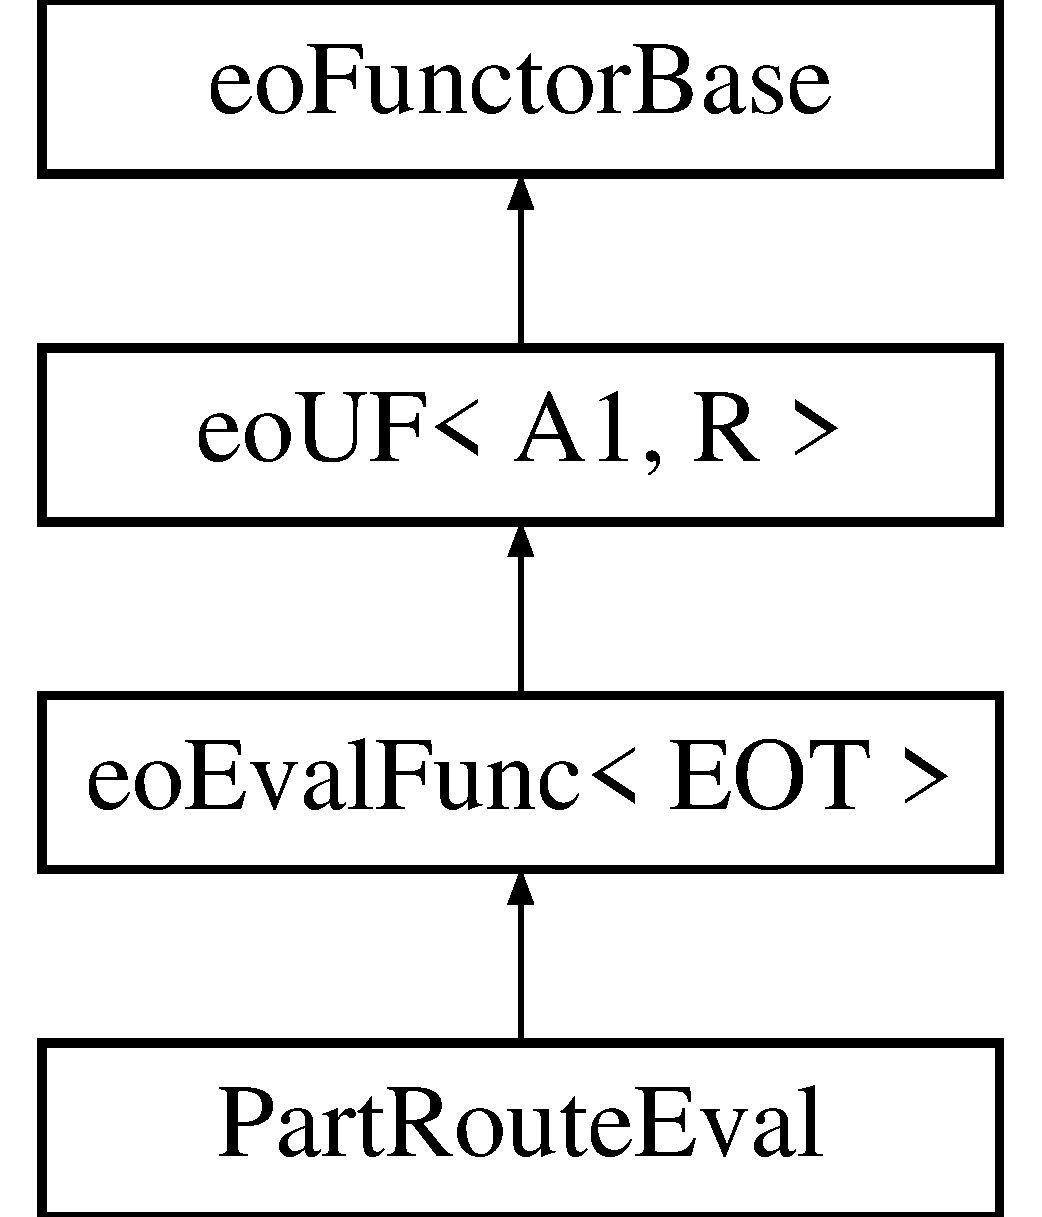
\includegraphics[height=4cm]{classPartRouteEval}
\end{center}
\end{figure}
\subsection*{Public Member Functions}
\begin{CompactItemize}
\item 
\hypertarget{classPartRouteEval_a331566b29bc3227f377004232f05491}{
\hyperlink{classPartRouteEval_a331566b29bc3227f377004232f05491}{Part\-Route\-Eval} (float \_\-\_\-from, float \_\-\_\-to)}
\label{classPartRouteEval_a331566b29bc3227f377004232f05491}

\begin{CompactList}\small\item\em Constructor. \item\end{CompactList}\item 
\hypertarget{classPartRouteEval_965fab875fb601f17934a6ece761beae}{
void \hyperlink{classPartRouteEval_965fab875fb601f17934a6ece761beae}{operator()} (\bf{Route} \&\_\-\_\-route)}
\label{classPartRouteEval_965fab875fb601f17934a6ece761beae}

\end{CompactItemize}
\subsection*{Private Attributes}
\begin{CompactItemize}
\item 
\hypertarget{classPartRouteEval_5bde722e66378b2570ae6c4b4f8df58e}{
float \hyperlink{classPartRouteEval_5bde722e66378b2570ae6c4b4f8df58e}{from}}
\label{classPartRouteEval_5bde722e66378b2570ae6c4b4f8df58e}

\item 
\hypertarget{classPartRouteEval_de53cc919faa498663f327b72c357da3}{
float \hyperlink{classPartRouteEval_de53cc919faa498663f327b72c357da3}{to}}
\label{classPartRouteEval_de53cc919faa498663f327b72c357da3}

\end{CompactItemize}


\subsection{Detailed Description}
Route Evaluator. 



Definition at line 45 of file part\_\-route\_\-eval.h.

The documentation for this class was generated from the following files:\begin{CompactItemize}
\item 
part\_\-route\_\-eval.h\item 
part\_\-route\_\-eval.cpp\end{CompactItemize}

\hypertarget{classRouteEval}{
\section{Route\-Eval Class Reference}
\label{classRouteEval}\index{RouteEval@{RouteEval}}
}
Inheritance diagram for Route\-Eval::\begin{figure}[H]
\begin{center}
\leavevmode
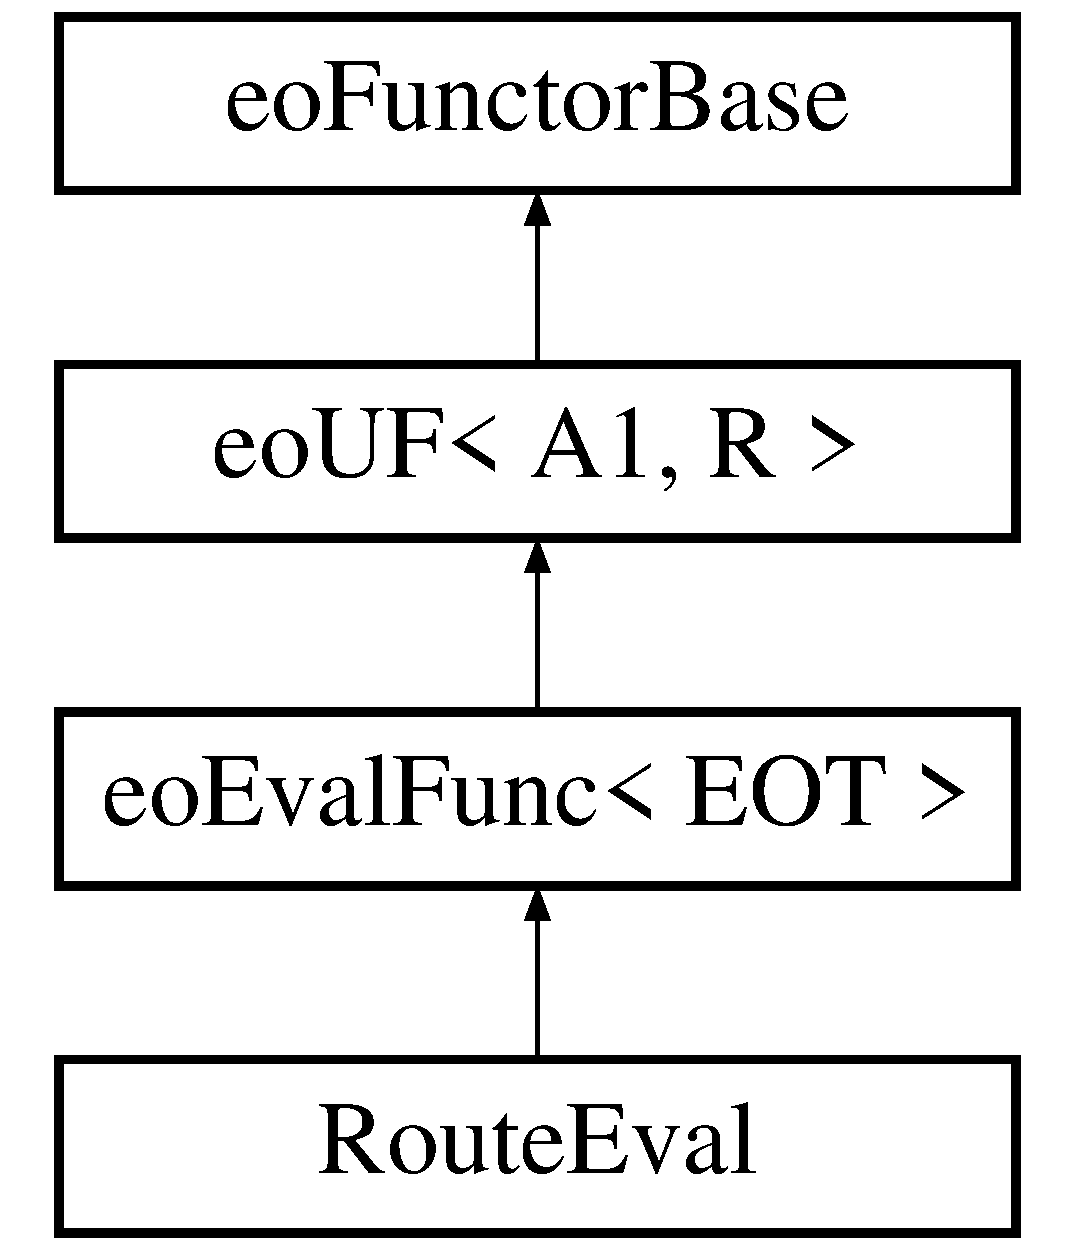
\includegraphics[height=4cm]{classRouteEval}
\end{center}
\end{figure}
\subsection*{Public Member Functions}
\begin{CompactItemize}
\item 
\hypertarget{classRouteEval_e10bbe6f792e6f44405953de4f703901}{
void \hyperlink{classRouteEval_e10bbe6f792e6f44405953de4f703901}{operator()} (\bf{Route} \&\_\-\_\-route)}
\label{classRouteEval_e10bbe6f792e6f44405953de4f703901}

\end{CompactItemize}


\subsection{Detailed Description}




Definition at line 44 of file route\_\-eval.h.

The documentation for this class was generated from the following files:\begin{CompactItemize}
\item 
route\_\-eval.h\item 
route\_\-eval.cpp\end{CompactItemize}

\hypertarget{classRouteInit}{
\section{Route\-Init Class Reference}
\label{classRouteInit}\index{RouteInit@{RouteInit}}
}
\subsection*{Public Member Functions}
\begin{CompactItemize}
\item 
\hypertarget{classRouteInit_b65a7137e114458faadb6a5510c001f7}{
void \hyperlink{classRouteInit_b65a7137e114458faadb6a5510c001f7}{operator()} (Route \&\_\-\_\-route)}
\label{classRouteInit_b65a7137e114458faadb6a5510c001f7}

\end{CompactItemize}


\subsection{Detailed Description}




Definition at line 16 of file route\_\-init.h.

The documentation for this class was generated from the following files:\begin{CompactItemize}
\item 
route\_\-init.h\item 
route\_\-init.cpp\end{CompactItemize}

\hypertarget{classTwoOpt}{
\section{Two\-Opt Class Reference}
\label{classTwoOpt}\index{TwoOpt@{TwoOpt}}
}
Inheritance diagram for Two\-Opt::\begin{figure}[H]
\begin{center}
\leavevmode
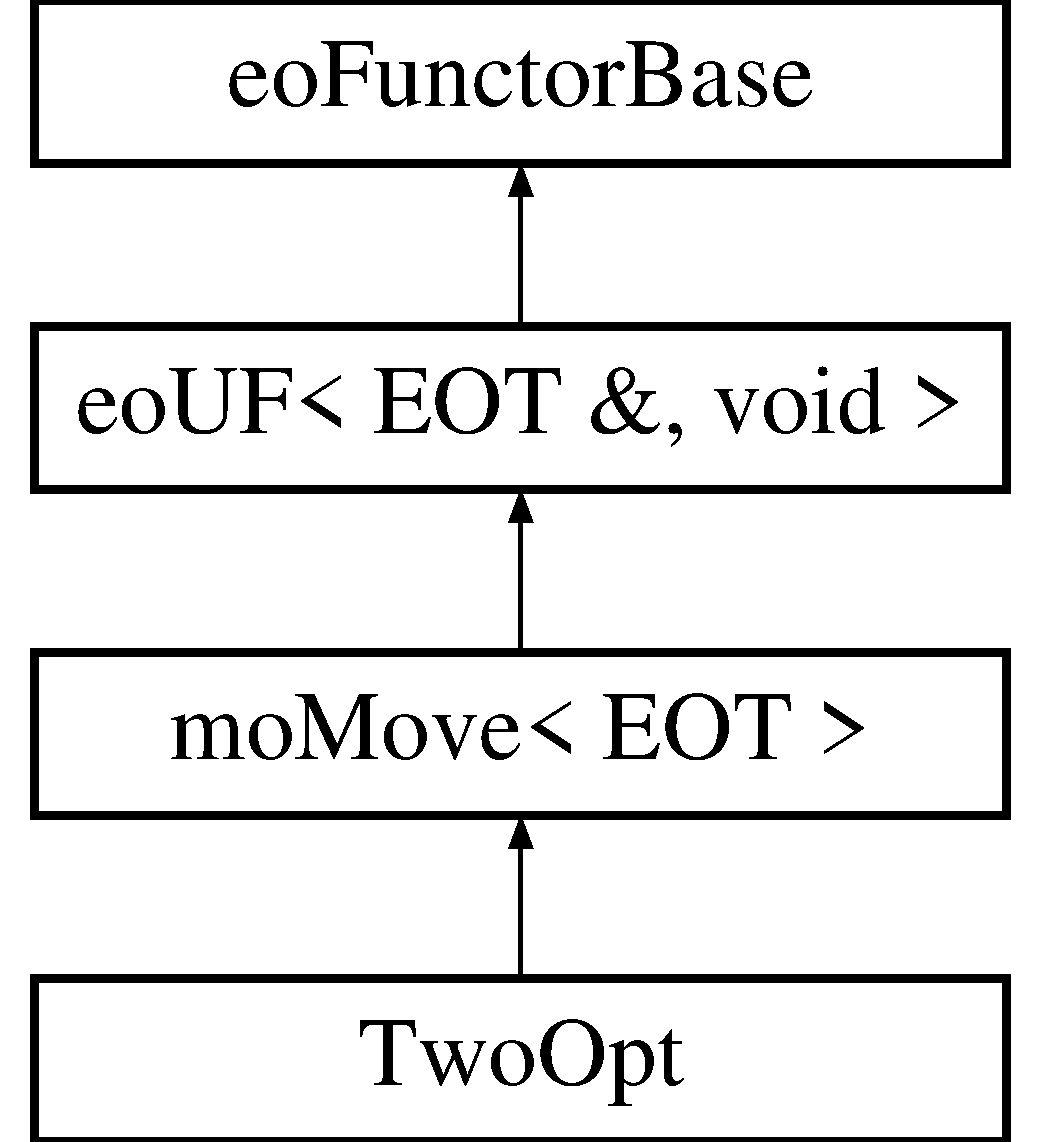
\includegraphics[height=2cm]{classTwoOpt}
\end{center}
\end{figure}
\subsection*{Public Member Functions}
\begin{CompactItemize}
\item 
\hypertarget{classTwoOpt_ff87d1649a33d42a6d64e8d314ed1af0}{
void \hyperlink{classTwoOpt_ff87d1649a33d42a6d64e8d314ed1af0}{operator()} (Route \&\_\-\_\-route)}
\label{classTwoOpt_ff87d1649a33d42a6d64e8d314ed1af0}

\end{CompactItemize}


\subsection{Detailed Description}




Definition at line 17 of file two\_\-opt.h.

The documentation for this class was generated from the following files:\begin{CompactItemize}
\item 
two\_\-opt.h\item 
two\_\-opt.cpp\end{CompactItemize}

\hypertarget{classTwoOptIncrEval}{
\section{Two\-Opt\-Incr\-Eval Class Reference}
\label{classTwoOptIncrEval}\index{TwoOptIncrEval@{TwoOptIncrEval}}
}
\subsection*{Public Member Functions}
\begin{CompactItemize}
\item 
\hypertarget{classTwoOptIncrEval_48500077e651c4c6152daef8a396be39}{
int \hyperlink{classTwoOptIncrEval_48500077e651c4c6152daef8a396be39}{operator()} (const \hyperlink{classTwoOpt}{Two\-Opt} \&\_\-\_\-move, const Route \&\_\-\_\-route)}
\label{classTwoOptIncrEval_48500077e651c4c6152daef8a396be39}

\end{CompactItemize}


\subsection{Detailed Description}




Definition at line 30 of file two\_\-opt\_\-incr\_\-eval.h.

The documentation for this class was generated from the following files:\begin{CompactItemize}
\item 
two\_\-opt\_\-incr\_\-eval.h\item 
two\_\-opt\_\-incr\_\-eval.cpp\end{CompactItemize}

\hypertarget{classTwoOptInit}{
\section{Two\-Opt\-Init Class Reference}
\label{classTwoOptInit}\index{TwoOptInit@{TwoOptInit}}
}
Inheritance diagram for Two\-Opt\-Init::\begin{figure}[H]
\begin{center}
\leavevmode
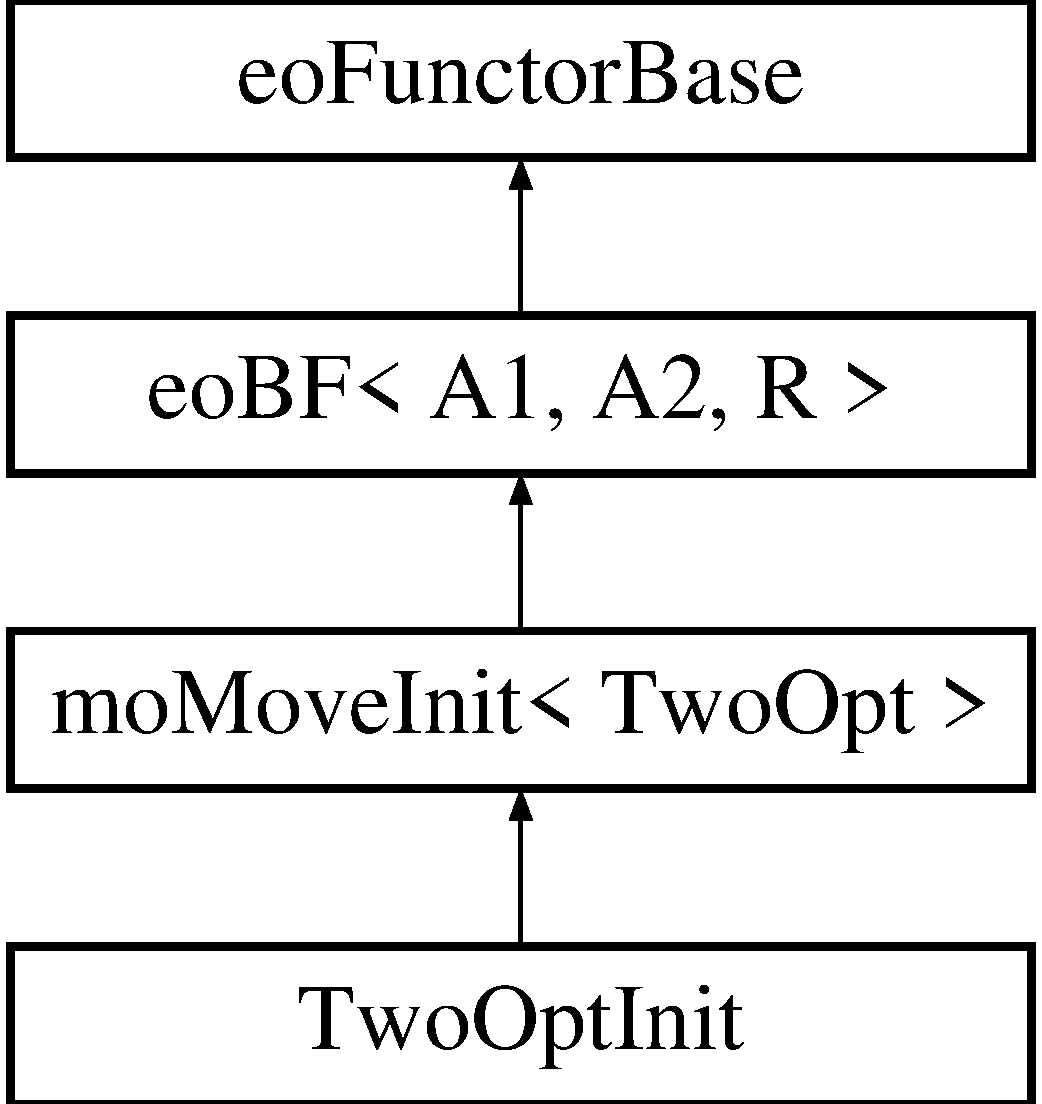
\includegraphics[height=4cm]{classTwoOptInit}
\end{center}
\end{figure}
\subsection*{Public Member Functions}
\begin{CompactItemize}
\item 
\hypertarget{classTwoOptInit_5bf6af064d37ebd955ffb5a623e78e1b}{
void \hyperlink{classTwoOptInit_5bf6af064d37ebd955ffb5a623e78e1b}{operator()} (\hyperlink{classTwoOpt}{Two\-Opt} \&\_\-\_\-move, const \bf{Route} \&\_\-\_\-route)}
\label{classTwoOptInit_5bf6af064d37ebd955ffb5a623e78e1b}

\end{CompactItemize}


\subsection{Detailed Description}




Definition at line 44 of file two\_\-opt\_\-init.h.

The documentation for this class was generated from the following files:\begin{CompactItemize}
\item 
two\_\-opt\_\-init.h\item 
two\_\-opt\_\-init.cpp\end{CompactItemize}

\hypertarget{classTwoOptNext}{
\section{Two\-Opt\-Next Class Reference}
\label{classTwoOptNext}\index{TwoOptNext@{TwoOptNext}}
}
Inheritance diagram for Two\-Opt\-Next::\begin{figure}[H]
\begin{center}
\leavevmode
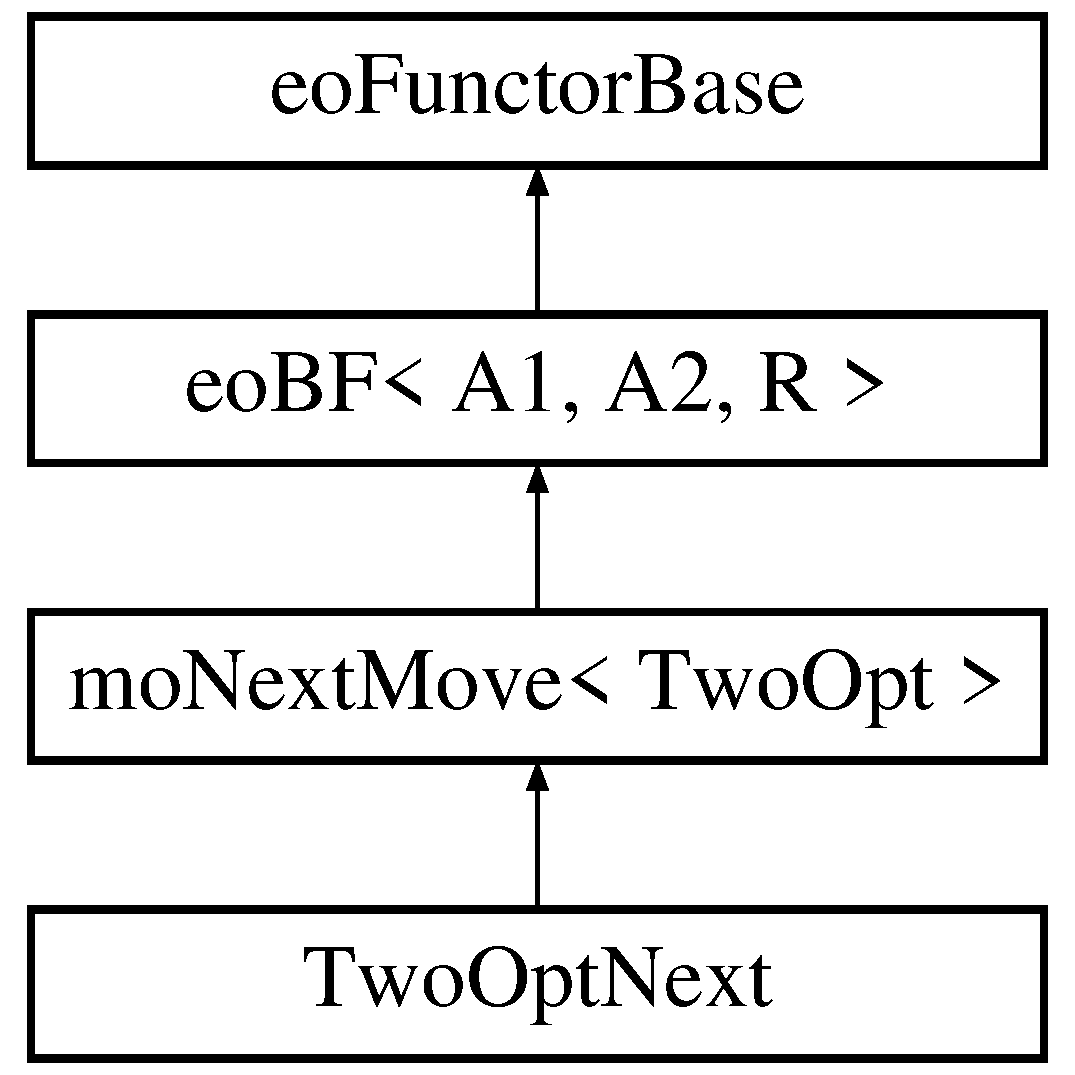
\includegraphics[height=4cm]{classTwoOptNext}
\end{center}
\end{figure}
\subsection*{Public Member Functions}
\begin{CompactItemize}
\item 
\hypertarget{classTwoOptNext_baf229b2e056f39ab971cf2ac66a833e}{
bool \hyperlink{classTwoOptNext_baf229b2e056f39ab971cf2ac66a833e}{operator()} (\hyperlink{classTwoOpt}{Two\-Opt} \&\_\-\_\-move, const \bf{Route} \&\_\-\_\-route)}
\label{classTwoOptNext_baf229b2e056f39ab971cf2ac66a833e}

\end{CompactItemize}


\subsection{Detailed Description}




Definition at line 44 of file two\_\-opt\_\-next.h.

The documentation for this class was generated from the following files:\begin{CompactItemize}
\item 
two\_\-opt\_\-next.h\item 
two\_\-opt\_\-next.cpp\end{CompactItemize}

\hypertarget{classTwoOptRand}{
\section{Two\-Opt\-Rand Class Reference}
\label{classTwoOptRand}\index{TwoOptRand@{TwoOptRand}}
}
\subsection*{Public Member Functions}
\begin{CompactItemize}
\item 
\hypertarget{classTwoOptRand_e2f362f359517c027f6f22fba0aab375}{
void \hyperlink{classTwoOptRand_e2f362f359517c027f6f22fba0aab375}{operator()} (\hyperlink{classTwoOpt}{Two\-Opt} \&\_\-\_\-move, const Route \&\_\-\_\-route)}
\label{classTwoOptRand_e2f362f359517c027f6f22fba0aab375}

\end{CompactItemize}


\subsection{Detailed Description}




Definition at line 16 of file two\_\-opt\_\-rand.h.

The documentation for this class was generated from the following files:\begin{CompactItemize}
\item 
two\_\-opt\_\-rand.h\item 
two\_\-opt\_\-rand.cpp\end{CompactItemize}

\printindex
\end{document}
